 % arara: xelatex: {shell: true}
% arara: biber
% arara: xelatex: {shell: true}
% arara: xelatex: {shell: true}

% Podklad k cvičení v předmětu BI-DPR
% autor: Ondřej Guth (ondrej.guth@fit.cvut.cz)
% (c) FIT ČVUT, 2018


\documentclass[a4paper]{article}
\usepackage{polyglossia}
\setmainlanguage{czech}
\usepackage{xevlna,xltxtra}
\usepackage{csquotes}
%\usepackage[style=german]{csquotes} % pro starší verze, kde není čeština

\usepackage[hidelinks]{hyperref}
\usepackage{graphicx}
\usepackage{minted}
\usepackage{xfrac}
\usepackage{nicefrac}
\usepackage[style=iso-numeric]{biblatex}

\title{MI-PAA\\
\large Úkol 1 -- zpráva\\}

\author{Tomáš Přeučil}

\begin{document}

\maketitle

%\tableofcontents

\section{Zadání úlohy}
	Úkolem bylo vytvořit program, který řeší problém batohu a to jak hrubou silou, tak pomocí jednoduché heuristiky -- poměru cen a vah.

\section{Použité prostředky}
	\subsection{Programovací jazyky a software}
		Úloha byla řešena v jazyce Python ve verzi 3.6 pod operačním systémem OS X 10.11.6. Program byl spouštěn z Bashe a tudíž pro spuštění nebylo využito žádné IDE.
		Pro měření času byla využita knihovna time a funkce \textit{time.process\_time()}. Jedná se o novinku od verze 3.3, která pracuje velmi podobně jako doporučovaná knihovna \textit{timeit}.
		
	\subsection{Konfigurace testovacího stroje}
		Testování bylo provedeno na MacBooku Pro 13", Early 2011, modelové číslo MC700LL/A. Stroj obsahuje CPU Intel Core i5 2415M (2,3~GHz) a 16~GB RAM. Jediný další rozdíl oproti výchozí konfiguraci je vyměněný disk (za SSD), což však v tomto případě nehraje roli.

\section{Rozbor možných variant řešení}
	V zadání bylo jasně dáno, že úkol by měl být řešen jak hrubou silou (pro malé instance) i pomocí heuristiky pracující s poměrem cena/váha.
	
	Nejjednodušším způsobem jak naprogramovat hrubou sílu je rekurzivní funkce, čehož bylo využito. Způsob tvorby heuristiky je zde jasně daný.

\section{Rámcový popis postupu řešení}
	Idea byla testovat hrubou sílu i heuristiku z jednoho pythonového programu. Proto byly vytvořeny dvě funkce, každá zpracovávající jednu část úlohy. Tyto funkce jsou pak volány z hlavního programu.
	
	Z důvodu rozumného měření času byla funkce pro heuristiku volána vždy tisíckrát a výsledný čas byl poté tisícem vydělen.
	
	Následný výstup byl zpracován pomocí awk a LibreOffice.

\section{Popis kostry algoritmu}
	Hrubá síla byla řešena pomocí rekurzivní funkce, tedy opravdu vyzkoušení všech různých možností. Základní ideou je vždy odebrat prvek z konce pole a funkci volat znovu -- buď bez prvku, nebo s ním a s o danou velikost sníženou kapacitou batohu.
	
	Heuristická funkce byla navržena tak, že je nejprve spočítána relativní hodnota věci, pole je podle této hodnoty seřazeno a věci jsou do batohu přidávány postupně, od nejvyšší relativní hodnoty. Cyklus je přerušen v případě, že zbývající kapacita batohu je nulová, jinak je zkoušeno vložení až všech předmětů.

\section{Naměřené výsledky}
	Hrubá síla se nepřekvapivě ukázala jako velmi neefektivní a již při 25 prvcích trval výpočet jedné instance 40-75 sekund. Proto byly instance s 25 prvky poslední, kde byla hrubá síla použita.
	
	Na druhou stranu doba výpočtu pomocí heuristiky byla i při instanci o 40 prvcích hluboko pod jednou sekundou. Naměřené časy výpočtu znázorňuje  graf \ref{cas} s logaritmickým měřítkem.
	\begin{figure}[h]
		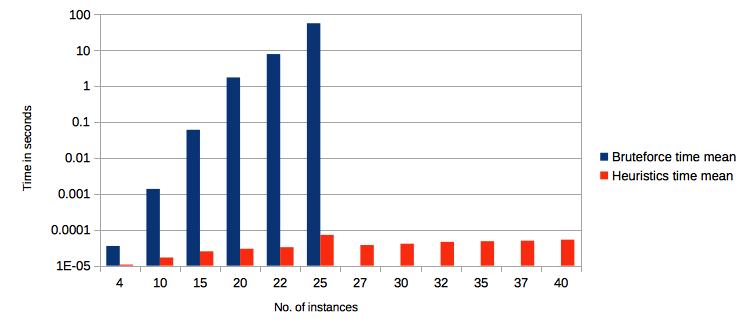
\includegraphics[width=0.9\textwidth]{cas_vypoctu.png} \caption{Časy výpočtu} \label{cas} 
	\end{figure}
	

	Co se týče relativní chyby, byla vypočítána dle doporučeného vzorce \begin{equation}\frac{optimum - aproximace}{optimum}\end{equation} a její průběh na instancích o velkostech 4-25 znázorňuje graf \ref{chyba}.
	
	\begin{figure}[ht]
		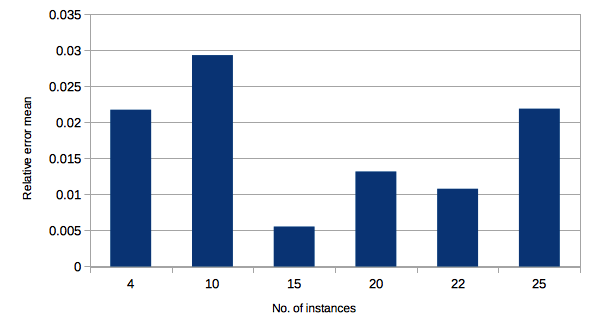
\includegraphics[width=0.9\textwidth]{relativni_chyba.png} \caption{Relativní chyba} \label{chyba}
	\end{figure}

%shrňte co jste naměřil
%porovnejte s předpoklady
%zkuste se vyjádřit k výsledku chyby, byť by to bylo i negativně
\section{Závěr}
	V rámci úkolu byly měřeny časy výpočtu pro hrubou sílu a jednoduchou heuristiku. Čas výpočtu pro hrubou sílu odpovídal předpokladu -- rostl exponenciálně. Z tohoto důvodu byl měřen čas jen pro instance o velikosti maximálně 25 prvků, jelikož výpočet větších instancí by nebyl časově reálný.
	
	Na stranu druhou byl z větší části potvrzen předpokládaný lineární růst času výpočtu při použití heuristiky. Je nutné říci že pouze z větší části, jelikož čas výpočtu pro instanci s 25 prvky tomuto předpokladu neodpovídá. Byla provedena kontrolní měření (včetně vypnutí garbage collectoru), ale výsledek byl stále stejný, jak je možné vidět na grafu \ref{cas}. Pravděpodobnou příčinnou této nepravidelnosti je nekonzistence vstupních dat. 
	
	Poslední měřenou hodnotou byla relativní chyba při výpočtu pomocí heuristiky. Ta byla měřena pouze pro instance do velikosti 25 prvků (včetně) a její nejvyšší hodnota byla necelá tři procenta, což je poměrně vysoké číslo. Pokud se vrátíme k původní podstatě problému, tak pokud zloděj kradl ve zlatnictví šperky v hodnotě milionu, tak právě přišel o třicet tisíc korun. Na stranu druhou ale mohl dokončit loupež dříve, než přijela policie. Z toho důvodu je nutné říci, že maximální naměřená hodnota chyby (3 \%) je vzhledem k úspoře času (dle mého názoru) uspokojivá. Dále se jedná \textit{pouze} o maximální naměřenou chybu, která, jak je možné vidět z grafu \ref{chyba}, může bát výrazně nižší.

\end{document}